\documentclass{beamer}
\usetheme{Warsaw}

\title{Parsing Natural Scenes and Natural Language with Recursive Neural Networks}
\author{Seungwoo Yoo}
\date{\today}

\begin{document}

\frame{\titlepage}

\section[Outline]{}
\frame{\tableofcontents}

\section{Introduction}
\subsection{Recursive structure}
\frame
{
  \frametitle{Parsing Natural Structural Examples}
  \begin{columns}
  \column{0.5\textwidth}
  \begin{figure}[ht]  
	  \begin{center}
		  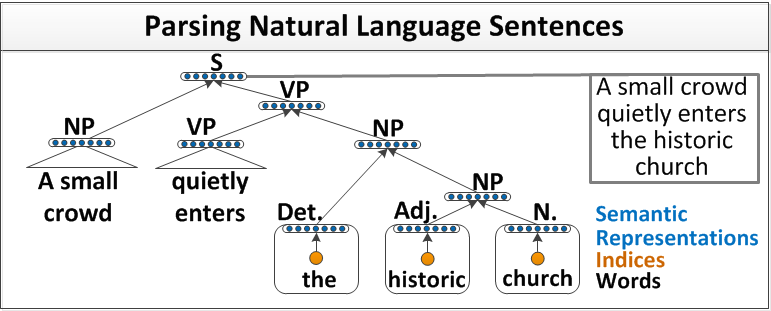
\includegraphics[width=2.1in]{images/fig1.png}   
	  \end{center}   
  \end{figure}
  \column{0.5\textwidth} 
  \begin{figure}[ht]
	  \begin{center}
		  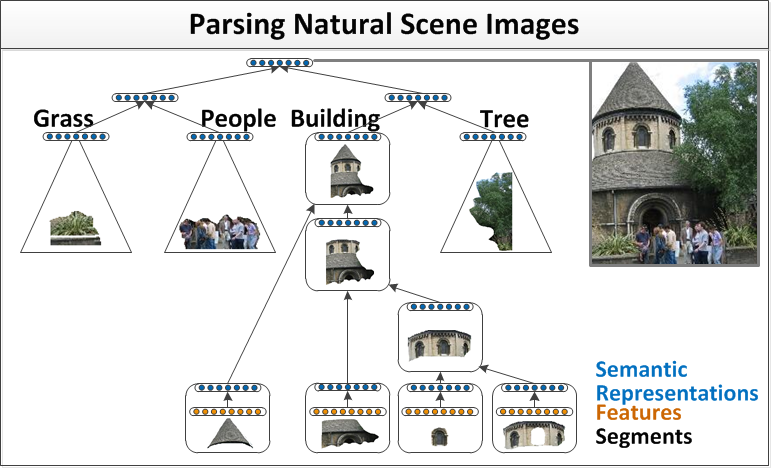
\includegraphics[width=2.1in]{images/fig2.png} 
	  \end{center}
  \end{figure}
  \end{columns}
}
\section{Algorithm Details}
\subsection{Mapping Segments and Words into Syntactico-Semantic Space}
\frame
{
}
\subsection{Recursiv Neural Networks for Structure Prediction}
\frame
{
}
\subsection{Max-Margin Estimation}
\frame
{
}
\subsection{Learning}
\frame
{
}
\section{Experimental Results}
\subsection{Scene Understanding: Segmentation and Annotation}
\frame
{
  \frametitle{Parsing Natural Scene Images}
  \begin{columns}
  \column{0.5\textwidth}
  \begin{figure}[ht]  
	  \begin{center}
		  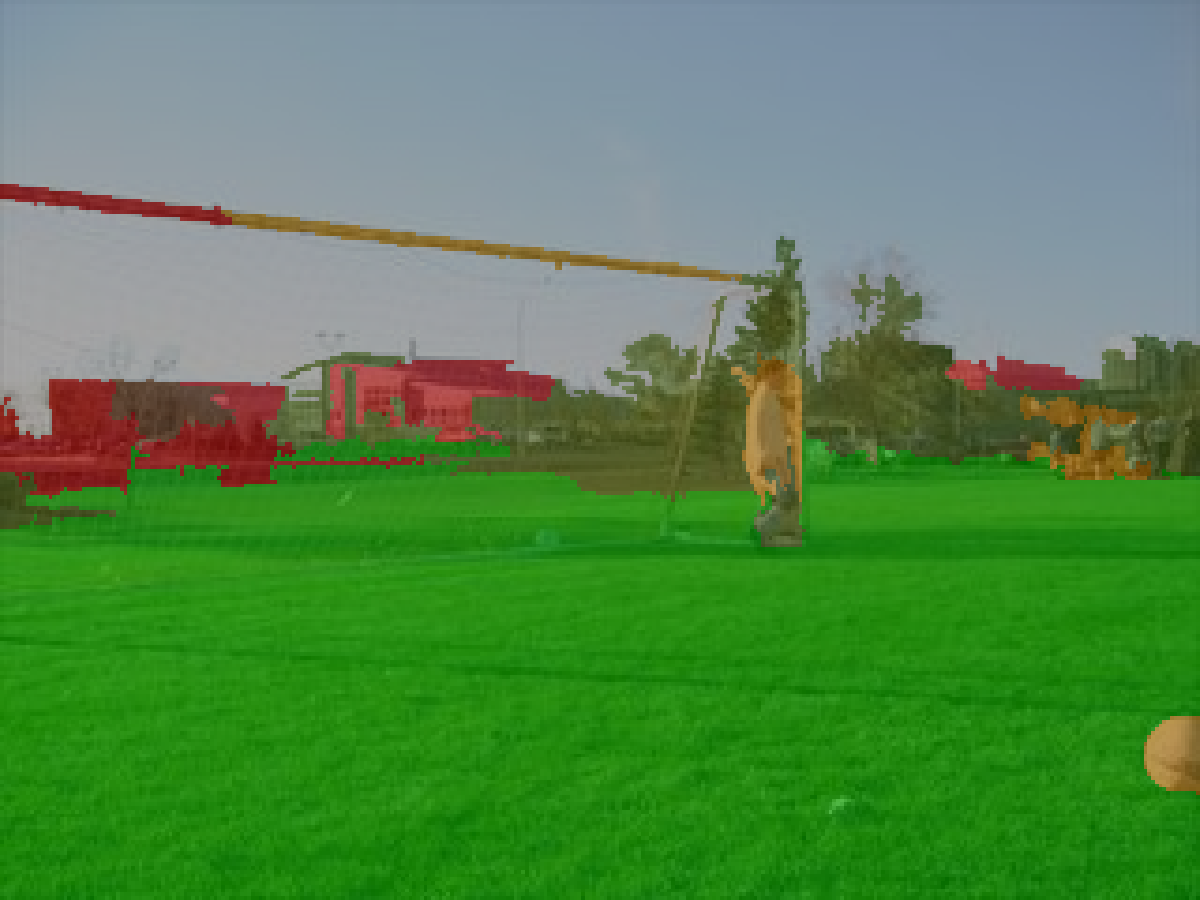
\includegraphics[width=2.1in]{images/ex1_ext.png}   
	  \end{center}   
  \end{figure}
  \column{0.5\textwidth} 
  \begin{figure}[ht]
	  \begin{center}
		  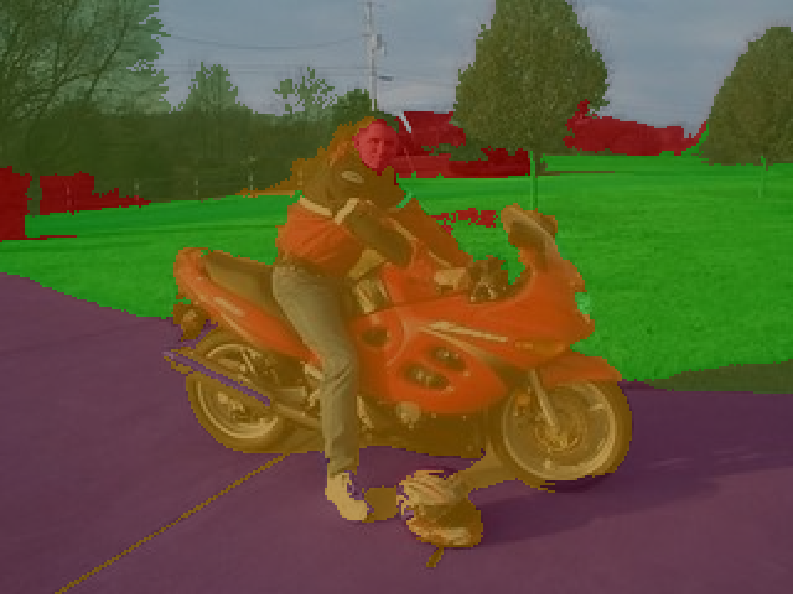
\includegraphics[width=2.1in]{images/ex1_ext2.png} 
	  \end{center}
  \end{figure}
  \end{columns}
}
\subsection{Scene Classification}
\frame
{
}
\subsection{Supervised Text Parsing}
\frame
{
}
\end{document}
